\chapter{Posterior Regularization}
Posterior regularization is an alternative way of clustering the phrases.
Unlike a Bayesian approach where intuitions about the data are 
expressed through the priors, 
posterior regularization imposes constraints 
on posterior distributions of the data.

In this chapter , we will introduce a basic clustering model with EM 
and look at shortcomings of the basic model. This will motivate us for
more complicated posterior regularized models.
\section{Phrase Clustering Model} 
As a brief recap, the clustering problem we are working with
is to label phrases with $K$ induced categories, where
$K$ is picked manually.
Phrases are obtained from bi-text data.
We also look at context
 words before and after
phrases as cues for clustering.
The relationship between phrases, contexts and categories are
represented with a generative model shown in 
Figure \ref{fig:EM}: a phrase picks a 
category and then that category generates the contex for the phrase.

\begin{figure}[h]
  \centering
  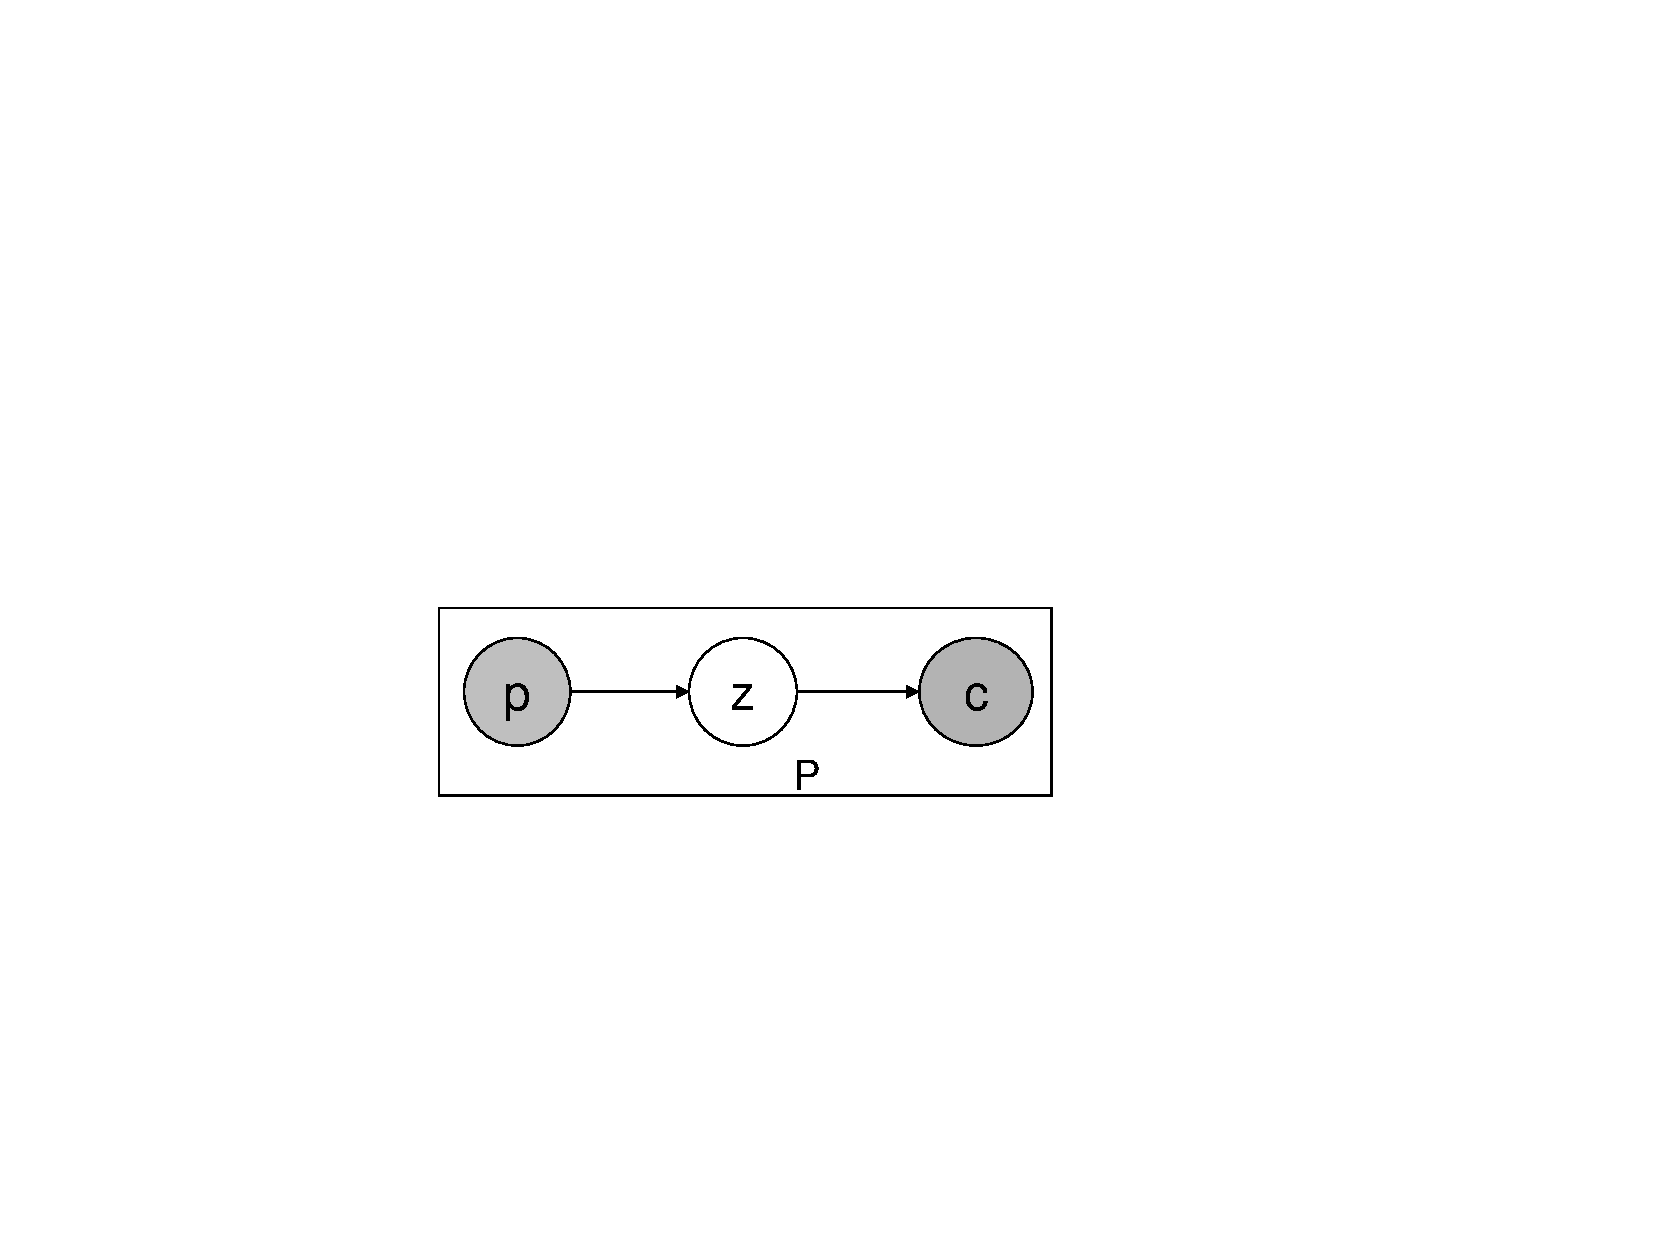
\includegraphics[width=3.0in]{pr-clustering/EMdigram}
  \caption{Basic Phrase Clustering Model}
  \label{fig:EM}
\end{figure}

The joint probability of a category $z$ and a context $\textbf{c}$ 
given a phrase $\textbf{p}$ is
\begin{equation}\label{eq:NBPost}
P(z,\textbf{c}|\textbf{p})=P(z|\textbf{p})P(\textbf{c}|z).
\end{equation}
$P(z|\textbf{p})$ is distribution of categories given a phrase.
This can be learned from data.
$P(\textbf{c}|z)$ is distribution of context given a category.
Since a context usually contains multiple slots for words, we further
decompose this distribution into independent distributions at
each slot. For example, suppose a context consists of two positions 
before and after the phrase. Denote these words as 
$c_{-2},c_{-1},c_1,c_2$.
Use $P_{-2},P_{-1},P_1,P_2$ to denote distributions of words at each 
position, $P(\textbf{c}|z)$ is decomposed as
\[
P(\textbf{c}|z)=P_{-2}(c_{-2}|z)P_{-1}
(c_{-1}|z)P_1(c_1|z)P_2(c_2|z).
\]
The posterior probability of a category given a phrase
and a context can be computed by normalizing the joint probability:
\[
P(z|\textbf{p},\textbf{c})=\frac{P(z,\textbf{c}|\textbf{p})}
{\sum_{i=1,K}P(i,\textbf{c}|\textbf{p})}.
\]
With the mechanisms to compute the posterior probabilities, we can 
apply expectation-maximization algorithm (EM)
 to learn all the probabilities.
EM algorithm maximizes the data likelihood
\[
\mathcal{L}=
\sum_{\textbf{p},\textbf{c}}
\log \sum_{z=1}^K P(z,\textbf{c}|\textbf{p})
\]
EM works by iterating between two steps:
E step computes posterior 
distributions according to Equation \ref{eq:NBPost},
M step updates model parameters with maximum likelihood
estimation as in Equation \ref{eq:MStep}.

\begin{equation}\label{eq:MStep}
\boldsymbol{\theta}=
\arg\max_{\boldsymbol{\theta}}
\sum_{\textbf{c},\textbf{p}}\sum_z
P(z|\textbf{p},\textbf{c},
\boldsymbol\theta^{old})\log
P(\textbf{c},\textbf{p}|z,\boldsymbol{\theta}).
\end{equation}

\section{Sparsity Constraints}\label{sec:pr-sparse}
A common linguistic intuition we have about the phrase 
clustering problem is that a phrase should be put into very
few categories, e.g. a verb phrase is unlikely to be used as 
a noun phrase. In other words, the categorization of
a phrase should be sparse.
The generative model we proposed above with EM
allows a phrase to be labelled with many tags. As we observed
from the output, EM is using more categories than we wanted for
each phrase.
Posterior regularization
provides a way to enforce sparsity \citep{ganchev:penn:2009}.
The general idea of posterior regularization is to modify
E-step of EM, so that instead of using posterior distribution
as the $q$ distribution directly, the nearest
$q$
in a constrained space is used
 as shown in Figure \ref{fig:EMPR}.

\begin{figure}[h]
  \centering
  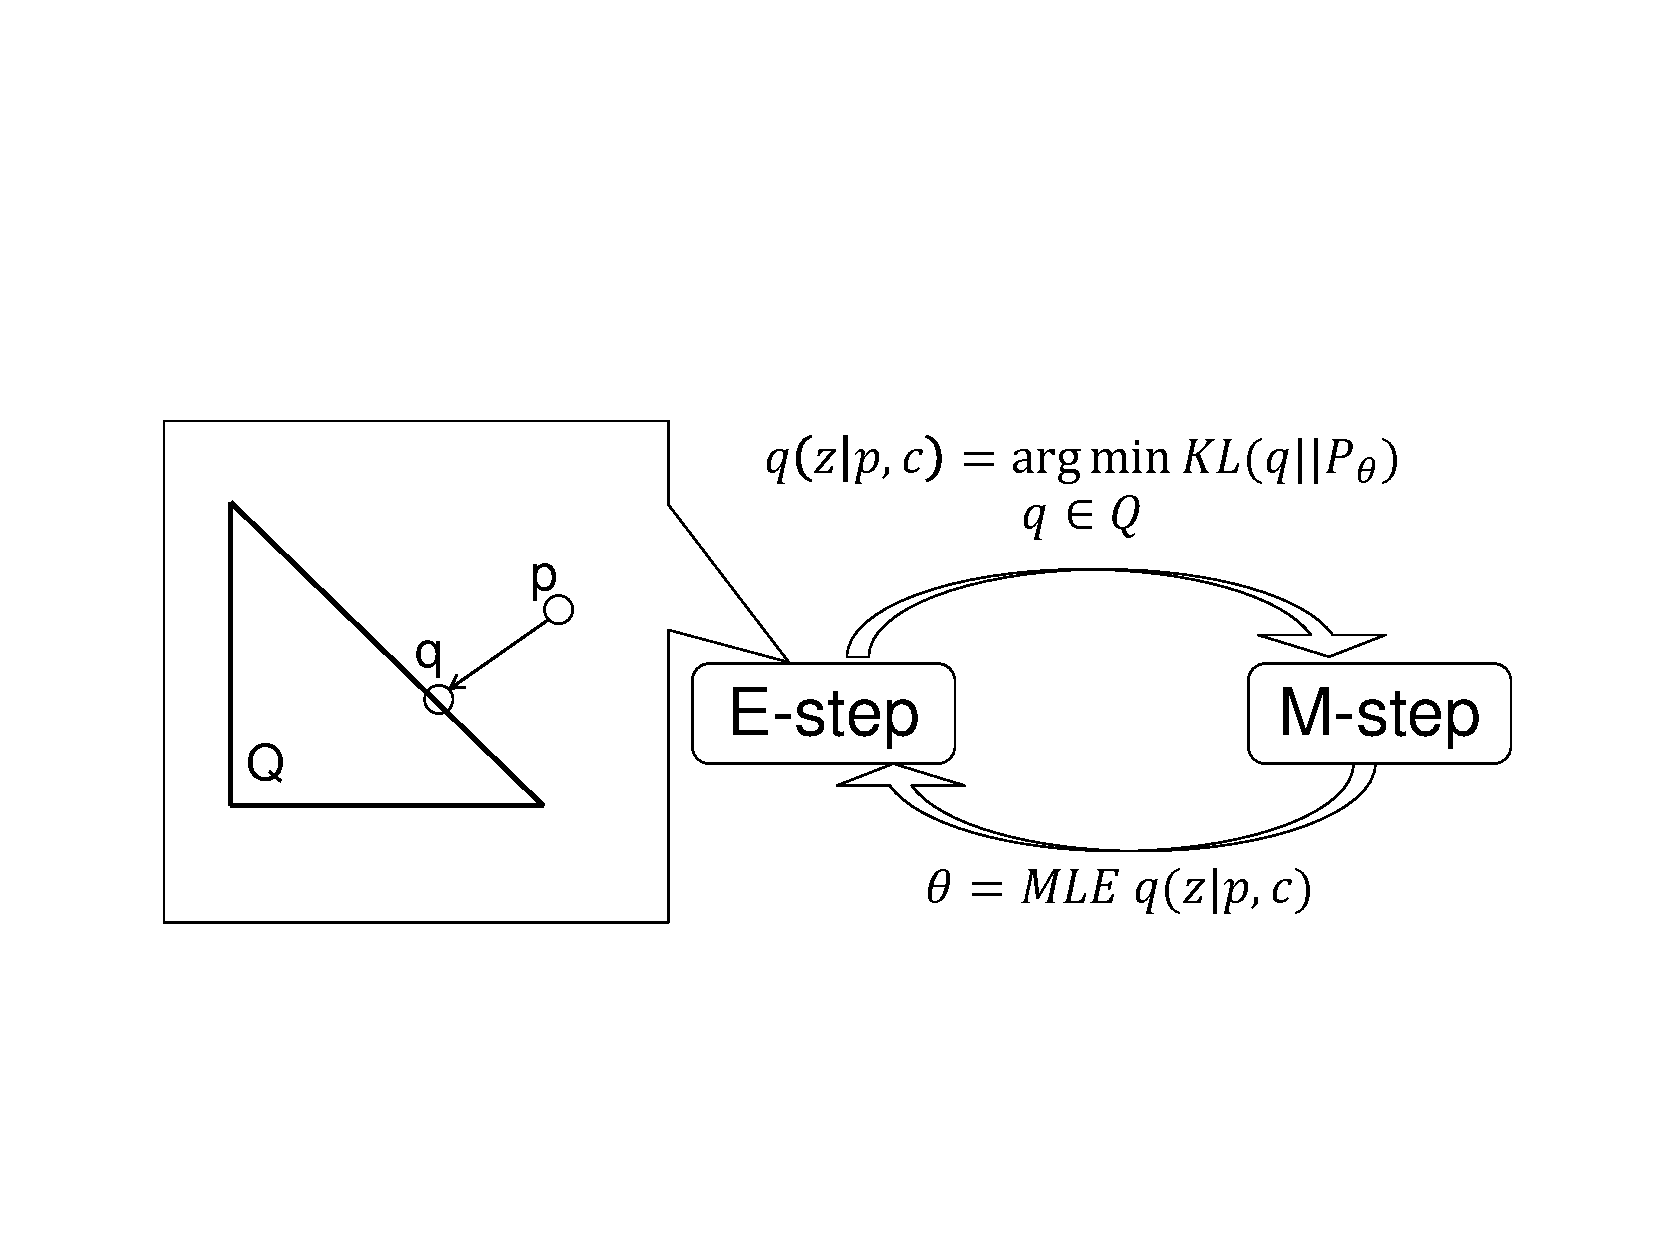
\includegraphics[width=3.5in]{pr-clustering/EMPR}
  \caption{EM with posterior regularization}
  \label{fig:EMPR}
\end{figure}

The constraint we use here is called $L_1/ L_\infty$
regularization in Ganchev's technical report. The notations
we use here largely follows Ganchev's.
In a more mathematical formulation, for each phrase $\textbf{p}$,
we want the quantity 
\begin{equation}\label{eq:sparsity}
\sum_{z=1}^K \max_i P(z|\textbf{p},\textbf{c}_i) 
\end{equation}
to be small, where $\textbf{c}_i$ is the context
appeared around the $i$th occurrence of phrase $\textbf{p}$
throughout the data. This quantity roughly equals 
the number of categories phrase $\textbf{p}$ uses.
It is minimized to $1$ if and only if
the posterior distributions $P(z|\textbf{p},\textbf{c}_i)$
are the same
for all
occurrences of $\textbf{p}$. That is ,
$\forall i,j$, 
$P(z|\textbf{p},\textbf{c}_i)=P(z|\textbf{p},\textbf{c}_j)$. 
For example, Table \ref{tab:sparse} compares two $L_1/L_{\infty}$
norms of phrases. The first phrase prefers multiple categories
under different contexts, the second phrase prefers
the same category under all contexts. The second phrase
has a much smaller $L_1/L_{\infty}$ norm.

\begin{table}[h]
  \label{tab:sparse}

  \centering
  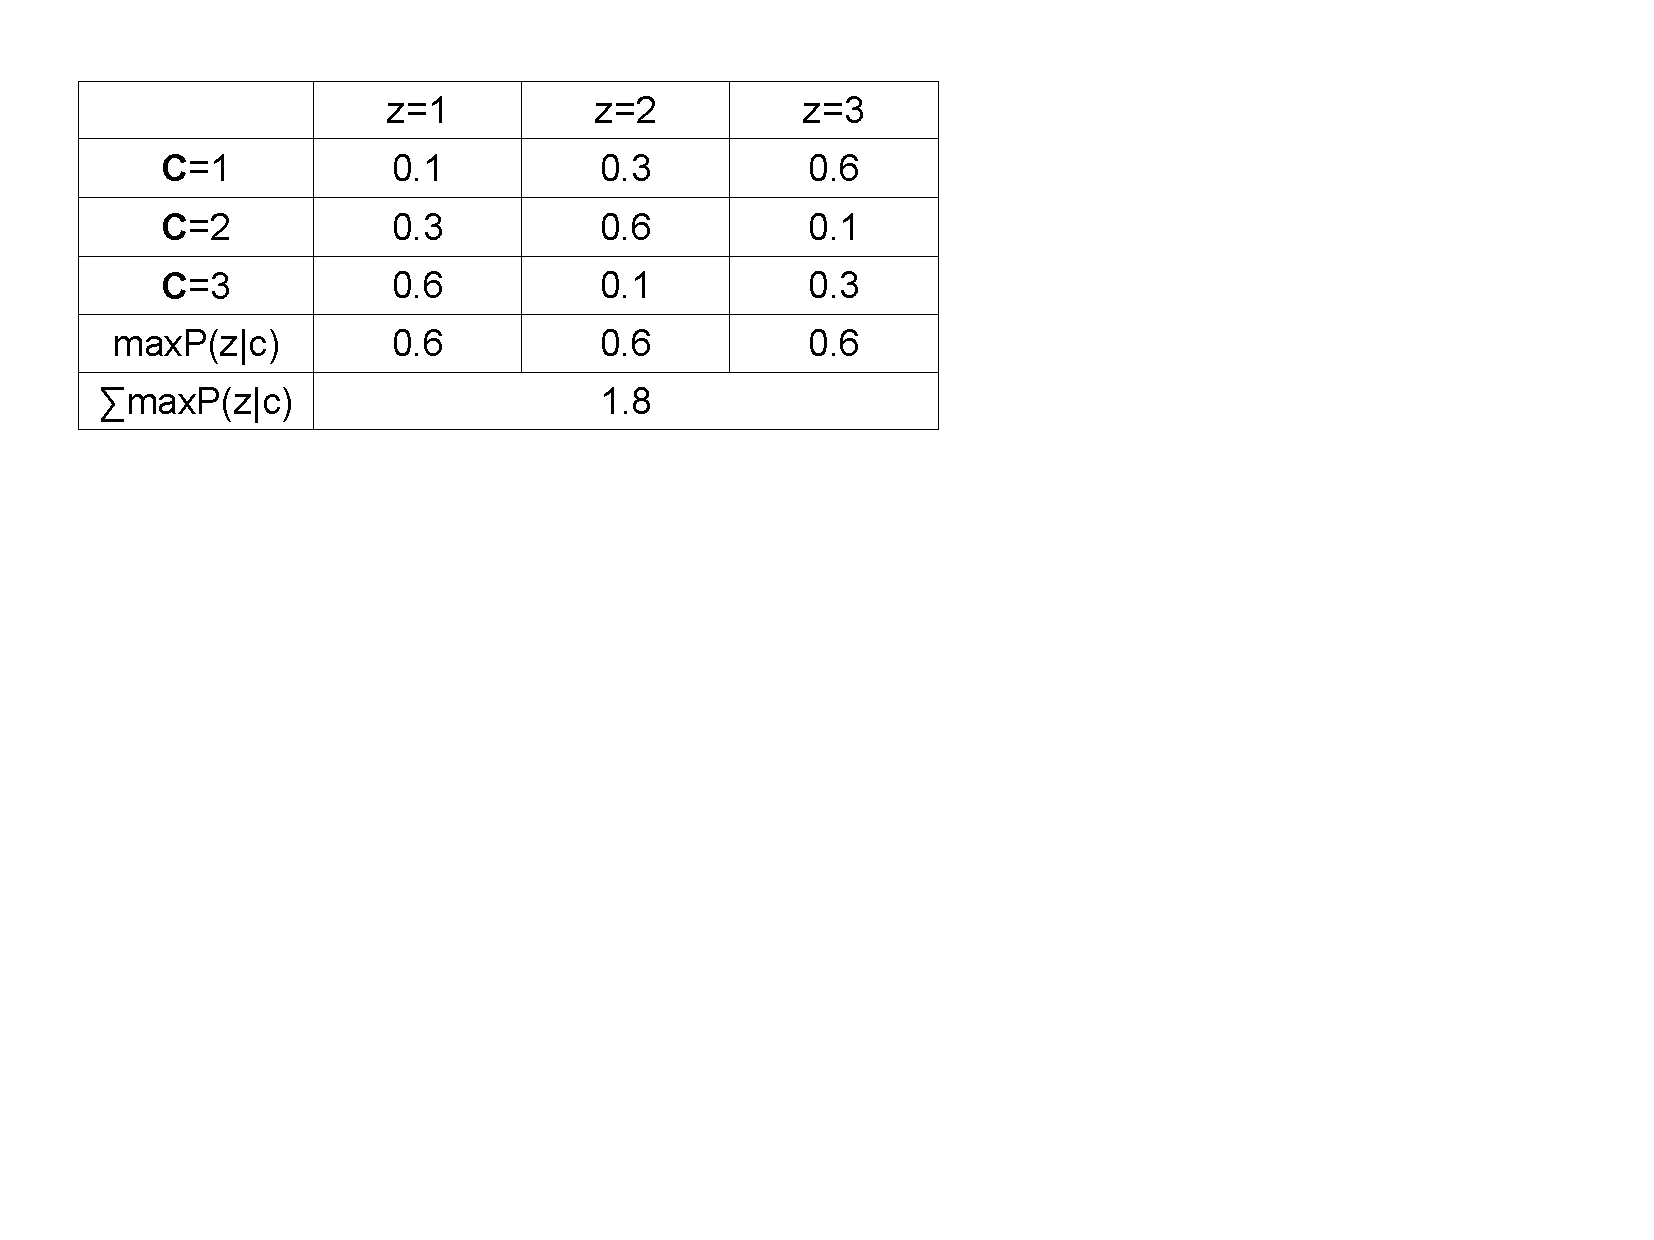
\includegraphics[width=3.5in]{pr-clustering/sparse0}
  \caption{$L_1/L_{\infty}$ norm of a phrase
  that prefers multiple categories}
  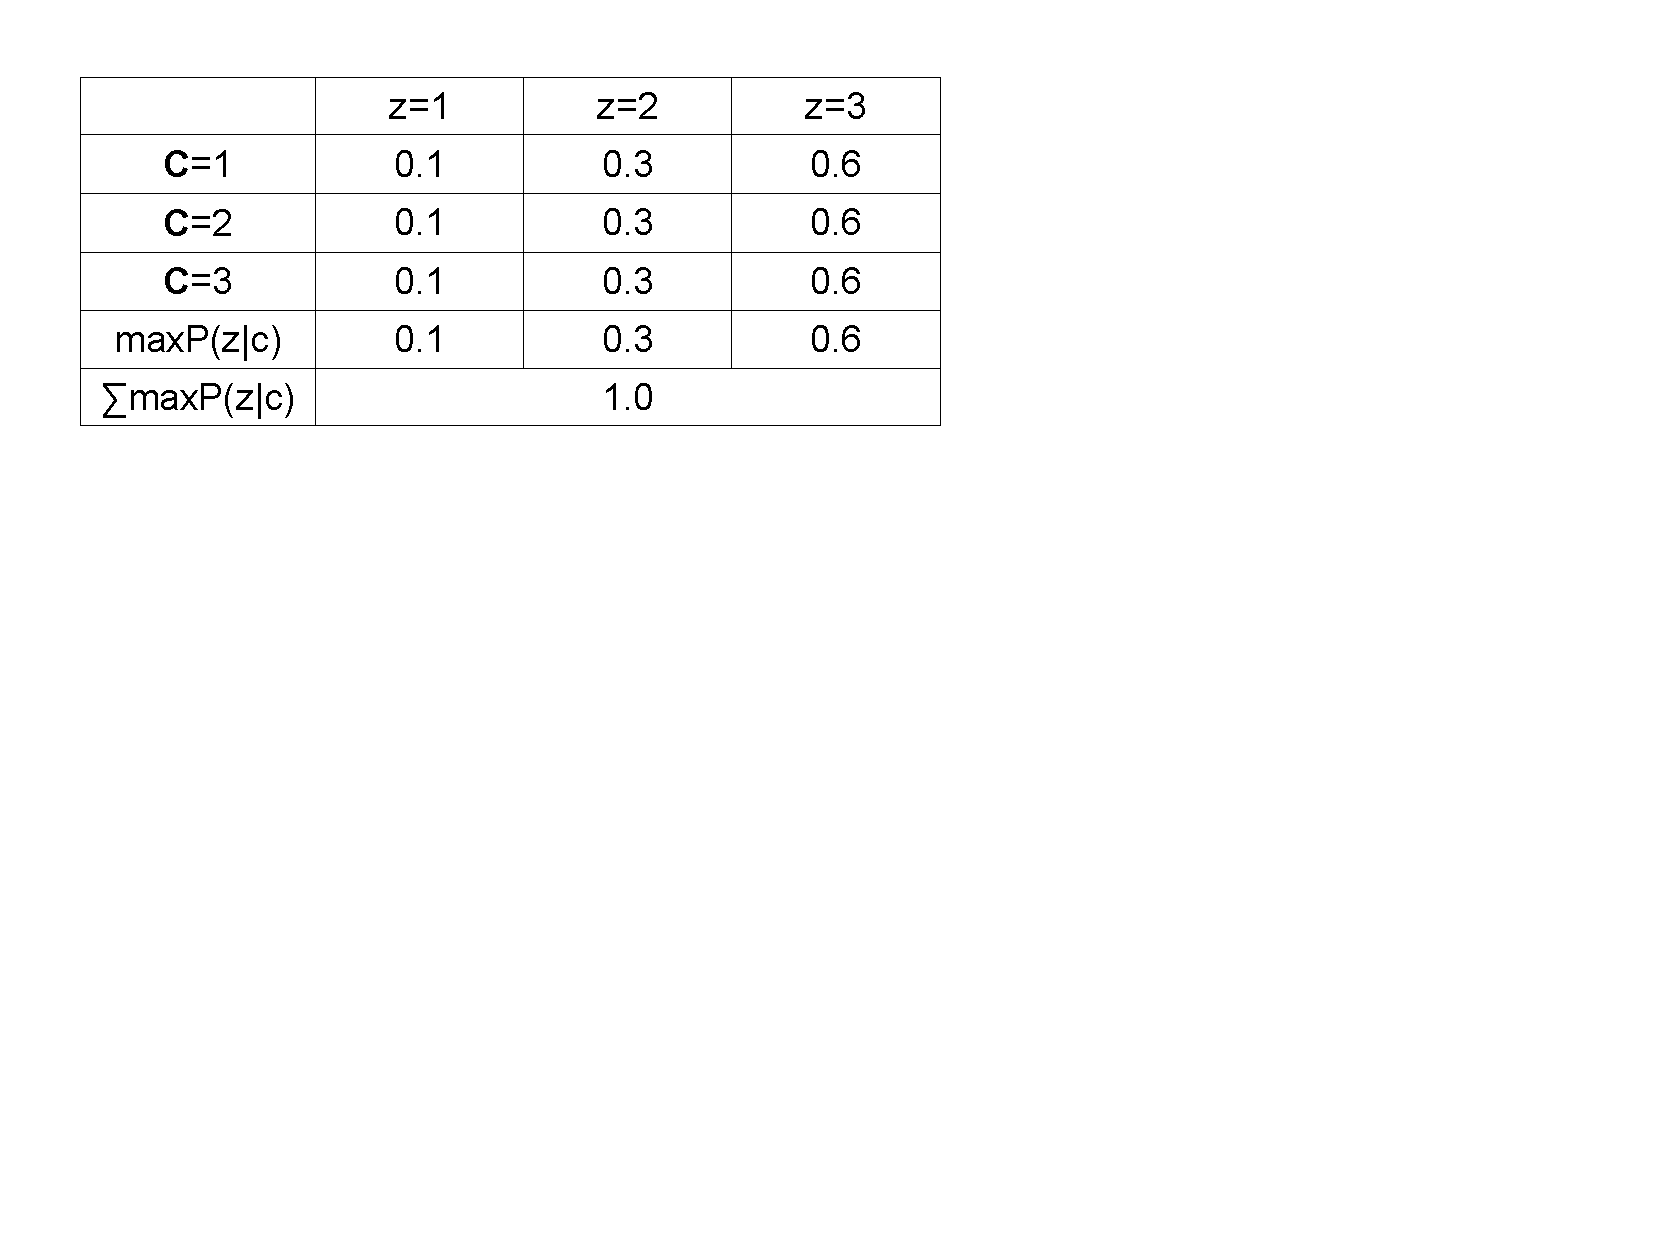
\includegraphics[width=3.5in]{pr-clustering/sparse1}
  \caption{$L_1/L_{\infty}$ norm of a phrase
  that prefers a single phrase}
\end{table}

Define feature functions for $i$th occurrence of phrase $\textbf{p}$
with category $j$,
as a function of category $z$:
\[
\phi_{\textbf{p}ij}(z)=
\begin{cases}
1\text{ if z=j}\\
0\text{ otherwise}
\end{cases}.
\]
For notation simplicity, for
each phrase category pair, 
define variables 
$e_{\textbf{p}z}$ to be 
$\max_i E_q[\phi_{\textbf{p}iz}]$. Note this is just
a different notation for the term in
Expression \ref{eq:sparsity}.

The objective we want to optimize becomes:
\[
\arg\min_{q,c_{\textbf{p}z}} KL(q||P_{\theta}) + 
\sigma \sum_{\textbf{p},z}e_{\textbf{p}z}
\]
\[
\text{ s.t. }\forall \textbf{p},z,
E_q[\phi_{\textbf{p}iz}]\leq e_{\textbf{p}z},
\]
where $\sigma$ is a constant to control
how strongly the soft constraint should
be enforced.
Using Lagrange Multipliers, this objective can
be optimized in its dual form,
for each phrase $\textbf{p}$:
\[
\arg\min_{\lambda\geq 0} \log 
(\sum_{z,i} P_\theta(z|\textbf{p},\textbf{c}_i)
\exp (-\lambda_{\textbf{p}iz}))
\]
\[
\text{ s.t. } \forall \textbf{p},z,
\sum_i \lambda_{\textbf{p}iz}\leq \sigma.
\]
This dual objective can be optimized with projected gradient
descent. Notice that each phrase has its own objective and
constraint. The $\lambda$s are not shared acrossed
phrases. Therefore we can optimize the objective
for each phrase separately. It is convenient for parallelizing
the algorithm. It also makes the objective easier to optimize.

The $q$ distribution we are looking for is then
\[
q_i(z)\propto P_{\theta}(z|\textbf{p},\textbf{c}_i)
\exp(\lambda_{\textbf{p}iz}).
\]
M-step can be performed as usual by replacing
$P(z|\textbf{p},\textbf{c},
\boldsymbol\theta^{old})$ with 
$q(z)$ in Equation \ref{eq:MStep}.

\section{Agreement Models}\label{sec:pr-agree}

Another type of constraint we used is agreement between
different models. The intuition is that if two models run
on the same dataset, it is desirable for them to give the same 
output. Suppose two models gives two posterior 
distributions of categories
$P_{\theta_1}(z|\textbf{p},\textbf{c})$,
$P_{\theta_2}(z|\textbf{p},\textbf{c})$. The
agreement constraint seeks posterior distributions
$q_1(z),q_2(z)$
such that $q_1(z)=q_2(z)$ while minimizing
the KL-divergence
$KL(q(z_1)q(z_2)||
P_{\theta_1}(z|\textbf{p},\textbf{c})
P_{\theta_1}(z|\textbf{p},\textbf{c}))$.
The solution to $q_1,q_2$ has a simple closed
form derived from Lagrange Multipliers shown in
Equation \ref{eq:AgreePost}.
\begin{equation}\label{eq:AgreePost}
q_1(z)=q_2(z)\propto 
\sqrt{P_{\theta_1}(z|\textbf{p},\textbf{c})
P_{\theta_1}(z|\textbf{p},\textbf{c})}
\end{equation}.

Since there is no reason to believe in that
phrases generates a category and then generate
a context, it is very natural to come up with a model
that generates in the reverse direction
as shown in Figure \ref{fig:EMreverse}. This model
and the original model should then follow the agreement 
constraint.
We also
took advantage of bi-text data and make models
learning from different languages to
agree with each other.

\begin{figure}[h]
  \centering
  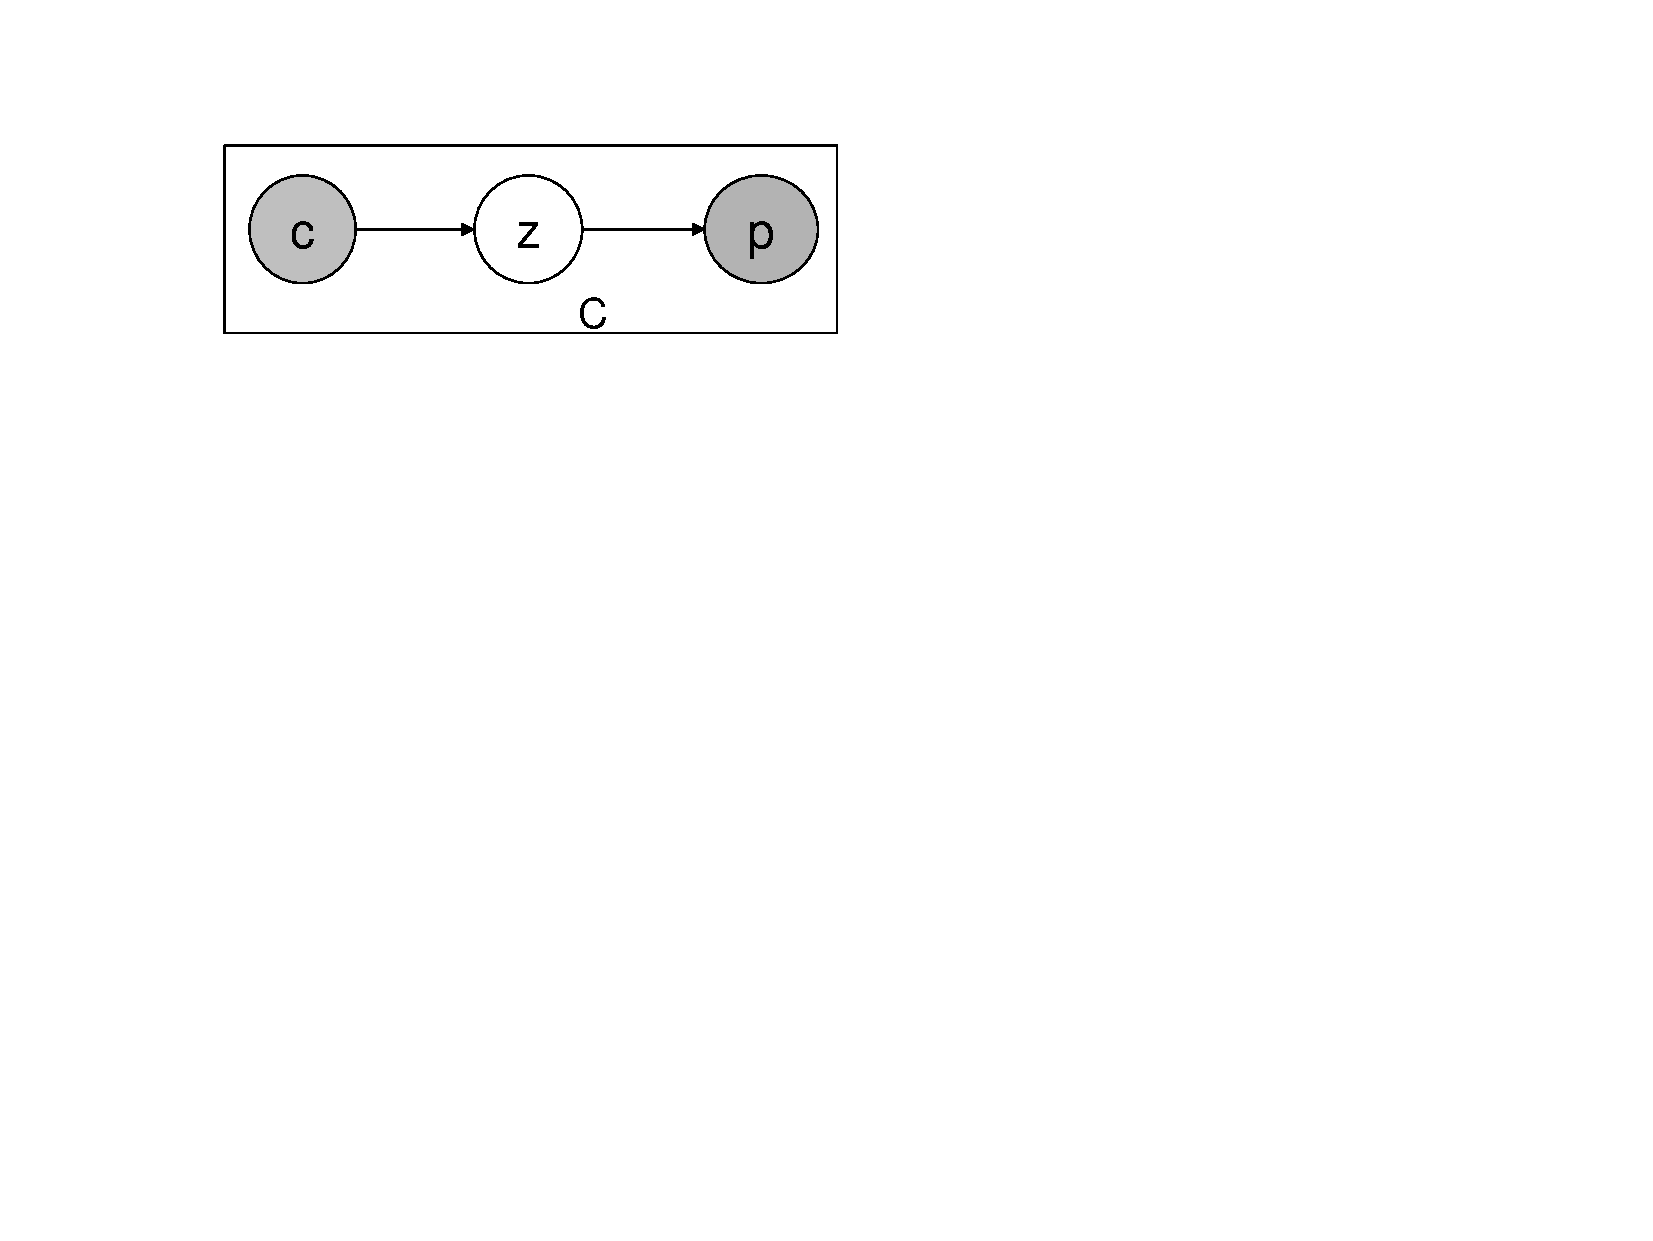
\includegraphics[width=3.0in]{pr-clustering/EMreverse}
  \caption{Generative Model in the reverse Direction}
  \label{fig:EMreverse}
\end{figure}

In the reversed model,
the posterior probability of the labelling of
a context $\textbf{c}$ with
phrase $\textbf{p}$ is 
\[
P(z|\textbf{c},\textbf{p})\propto 
P(z|\textbf{c})P(\textbf{p}|z).
\]
Since a phrase contains a variable number of words,
we only look at the first and last word of
a phrase. That is $P(\textbf{p}|z)=P_l(p_l|z)P_r(p_r|z)$,
where $P_l$ and $P_r$
denotes distributions for words in the first and last position
, $p_l$ and $p_r$ are words in the first and last position.

The implementation of agreement models again ends up making
a small change to E-step. The $q$ distribution for
a phrase $\textbf{p}$ and a context $\textbf{c}$ 
is given by Equation \ref{eq:AgreePost}.
In M-step, both models should update their parameters with $q$ distribution computed as above.
This modified EM is proven to
maximizes the objective:
\[
\mathcal{L}_1+
\mathcal{L}_2+
\sum_{\textbf{p},\textbf{c}}
\log\sum_z\sqrt{P_{\theta_1}(z|\textbf{p},\textbf{c})
P_{\theta_2}(z|\textbf{p},\textbf{c})},
\]
where $\mathcal{L}_1$ and $\mathcal{L}_2$
are log-likelihoods of
each individual model.
\section{Experiments}
As a sanity check, we looked at a few examples produced by
the basic model (EM) 
and the posterior regularization (PR) model
with sparsity constraints. Table \ref{tab:EMVSPR}
shows a few examples.

\begin{table}[h]
  \centering
  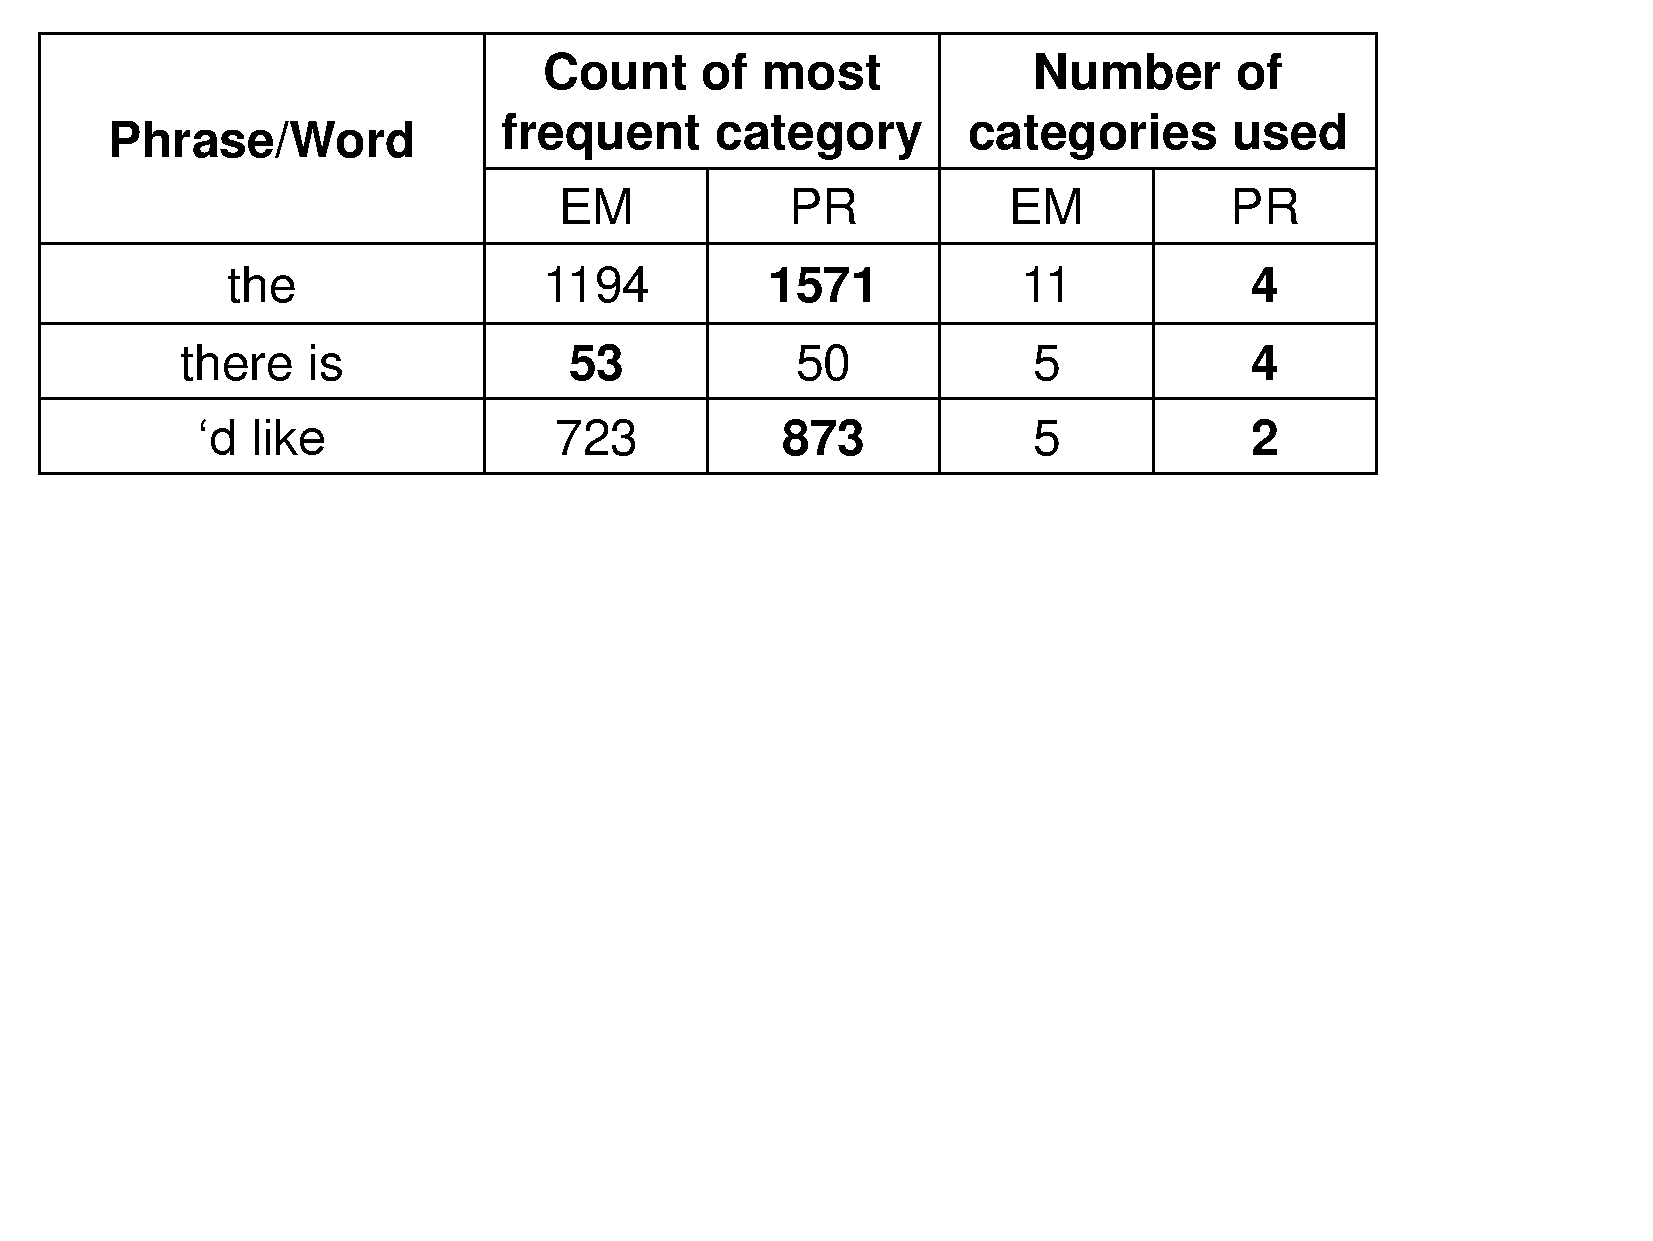
\includegraphics[width=3.5in]{pr-clustering/EMVSPR}
  \caption[A few examples comparing EM and PR]
  {A few examples comparing EM and PR. 
    Count of most frequent category shows how 
    many instances of a phrase are concentrated on 
    the single most frequent tag. 
    Number of categories shows how many categories
    a phrase is labelled with. By experience as mentioned before, 
    we want a phrase to use fewer categories. 
	These numbers are fair indicators of sparsity.
    }
  \label{tab:EMVSPR}
\end{table}

The models are formally evaluated with two kinds
of metrics. We feed the clustering output
through the whole translation pipeline 
to obtain a BLEU score. We also came up 
with an intrinsic evaluation of clustering quality
by comparing against a supervised CFG parser trained on the
tree bank.

We are mainly working on Urdu-English language pair. 
Urdu has very 
different word ordering from English. 
This leaves us room for improvement over
phrase-based systems.
Here in Table \ref{tab:results} 
we show BLEU scores as well as
conditional entropy for each of the models above
on Urdu data. Conditional entropy is computed
as the entropy of ``gold'' labelling given
the predicted clustering. ``Gold'' labelling
distribution
is obtained from Collins parser
trained on Penn Treebank. Since not
all phrases are constituents, we ignored
phrases that don't correspond to any constituents.

We conducted experiments with various data pre-processing
and tried different models. Number of phrase categories
is fixed at $25$. We chose to only look at
the target side language. The context is set
to be $1$ word to the left and to the right of the phrase.
We chose such a setting because it emperically works better
in the pipeline than other variations. This is also
the case for non-parametric methods. The models as we discussed
in previous sections are EM, EM with sparsity constraint, 
agreement of two models in reverse directions and agreement
of two models trained on two languages. We tried our models
with word classes as well. In the context, each word is
replaced with a word class unsupervisedly learned from the data.
The results are shown in Table \ref{tab:results}.

\begin{table}[h]
  \centering
  \begin{tabular}{ |*{4}{c|} }
    \hline
    \multicolumn{2}{|c|}{model} & BLEU & H(Gold$|$Predicted)\\
    \hline
    \multicolumn{2}{|c|}{hiero} & 21.1 & 5.77\\
    \multicolumn{2}{|c|}{hiero+POS} & 22.3 & 1.00 \\
    \multicolumn{2}{|c|}{SAMT} & 24.5 & 0.00 \\
    \hline
	\multirow{2}{*}{EM} & words & 20.9 & 2.85 \\
	& word classes & 21.54 & 2.86 \\ \hline
    \multirow{2}{*}{PR $\sigma=100$}&words & 21.1 & 2.56 \\
	&word classes & 21.7 & 2.36 \\ \hline
    \multirow{2}{*}{agree language}&word & 21.7 & 2.80 \\
	&word classes & 21.4 & 2.69\\ \hline
    \multirow{2}{*}{agree direction}&word & 21.6 & 2.48\\
	&word classes &22.1 &2.36 \\ \hline
   \multirow{2}{*}{non-parametric}&word & 22.0 & 2.86\\
	& word classes&22.3&2.27\\ 
    \hline
  \end{tabular}
    \caption
  {Evaluation of PR models.
	Left column shows BLEU scores
	through the translation pipeline.
	Right columns shows conditional entropy
	of the 
    }
  \label{tab:results}
\end{table}

In Table \ref{tab:results}, the first three rows
are baseline system. The rest are developed in the workshop.
Hiero is hierachical phrase-based
model with 1 category in all of its SCFG rules. Hiero+POS
is hiero with all words labelled with their POS tags.
SAMT is a syntax based system with a supervised
parser trained on Treebank. EM is the first model mentioned
in the beginning of this chapter. PR $\sigma=100$ is 
posterior regularization model with sparsity constraint
explained in Section \ref{sec:pr-sparse}.
$\sigma$ is the constant controls strongness of the constraint.
We picked $\sigma$ by trying different values ranging from 
$1$ to $100$.
Agree language and agree direction are models with agreement 
constraints mentioned in Section \ref{sec:pr-agree}. Non-parametric
is non-parametric model introduced in the previous chapter.
\section{Conclusion}
The posterior regularization framework has a solid theoretical foundation.
It is shown mathematically to balance between constraint and likelihood.
In our experiments,
we used it to enforce sparsity constraint and agreement constraint and
achieved results comparable to non-parametric method that enforces
sparcity through priors. The algorithm is fairly fast if the constraint
can be decomposed into smaller pieces and compute separately. In our case,
the sparsity constraint for phrases can be decomposed into one small optimization
procedure for each phrase. In practice, our algorithm is much 
faster than non-parametric models with Gibbs sampling inference. 
The agreement
models are even faster because they are performing almost the same amount
of computation as the simple models trained with EM.
